% Első előadás

\chapter{Intel Core 2 család}

\section{Kategorizálás}
A Core 2 családot 4 csoportra oszthatjuk:
\begin{itemize}
    \item szerverek (e3, e5, e7, Platinum, Gold)
    \item high-end desktopok (i7, i9)
    \item desktopok, laptopok (i3, i5, i7), összefoglalva kliensek
    \item mobilok (Atom - 2016-ban visszavonva)
\end{itemize}

A magok száma kategóriánként változik: szerverek max. 28, HEDT max. 18, desktopok 2-10 + grafika, mobilok max. 10 + grafika.
A magok számával a lapkaméret is nő, a szerverek nagyobbak a klienseknél és a mobiloknál.

\section{Kliens processzorok fejlődése}
\subsection{Magok száma}
A többmagos fejlődést a Pentium D indította el, de ez még nem valódi kétmagos processzor volt, mivel két, egymagos lapkát tokoztak egybe.
Ezután a Core 2 valósított meg 2 magot egy lapkán.
A Core 2 Quad 2 db 2 magos lapkát tokozott egybe.
A Nehalemmel már egy lapkán 4 mag lehetett.

Később megjelent a grafika, egy harmadik, egybetokozott grafikai maggal.
Eztuán sokáig nem történt semmi, a magok száma maximum 4 maradt.
2017-ben, hogy konkurenciát nyújtsanak az AMD-nek, emelték a magok számát.
A 10 nm-es rendszerek megjelenésekor az Intel nem követte a magszám növekedés irányát, először 2, aztán 4 magot alkalmazott.

\subsection{Memória csatornák}
A memória csatorna szám végig 2 maradt.
Bár a magok számának növekedésével gyorsabb memória hozzáférésre is szükség volt, a memóriák fejlődése ellensúlyozta azt, hogy nem lett több csatorna.

\subsection{Memória vezérlő elhelyezése}
A Nehalem előtt a memóriavezérlőt az északi hídra helyezték.
Hátránya, hogy az északi híd és a processzor közötti kapcsolatot terheli a memória forgalma.
Ez főleg több processzoros rendszerekben negatívum, mivel az északi híd ekkor komolyan korlátozza a memória sávszélességét.
Tehát a processzorszám növekedésével a memória nem skálázódik.
Ezért a Nehalemtől a memória közvetlenül a processzorhoz csatlakozik (a lapkán lévő vezérlőhöz), ami rövidebb utakat és tehermentesített északi hidat jelent (\ref{fig:mc}. ábra).
Előny, hogy processzoronként külön memória kapcsolat létezhet, azaz skálázódik a processzorszámmal.
\begin{figure}[H]
    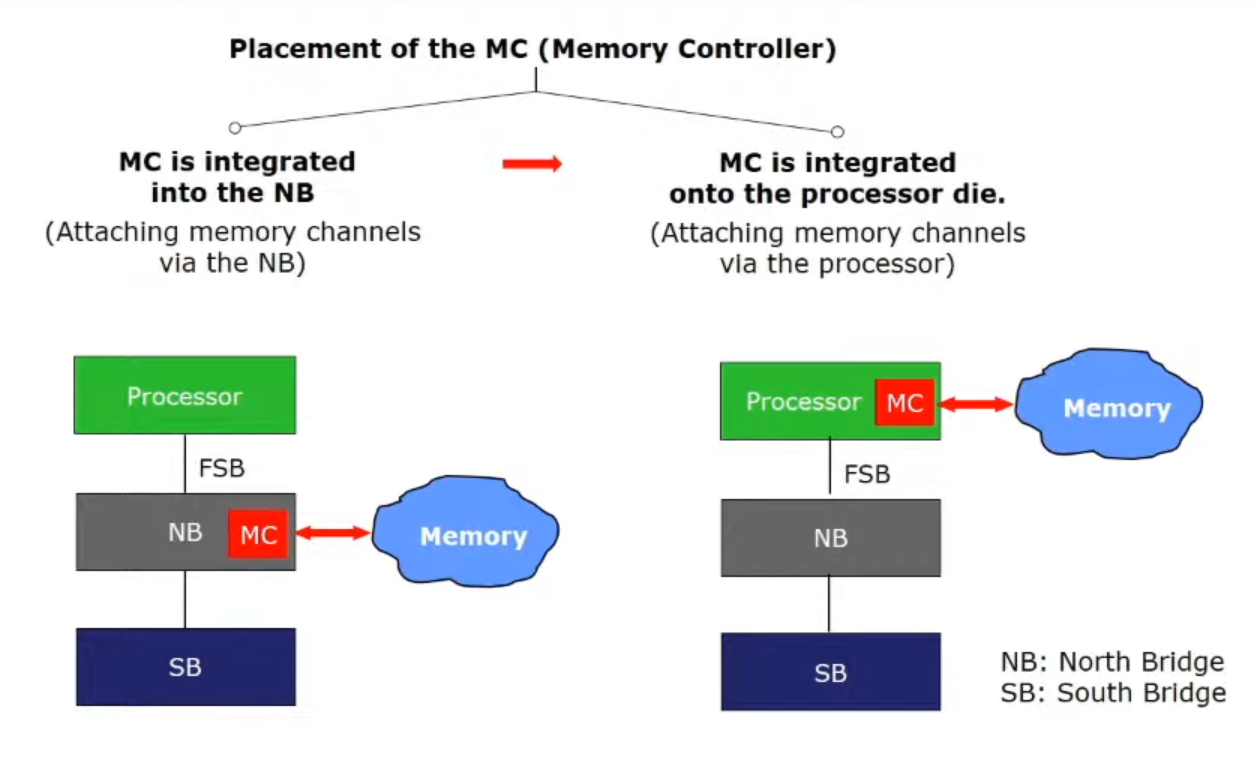
\includegraphics[width=\textwidth]{mc}
    \centering
    \caption{Memória kontrollek elhelyezkedése}
    \label{fig:mc}
\end{figure}
Később az északi híd egybeolvadt a délivel, amit periféria vezérlőnek neveztek el.

\subsection{Memória sebessége}
A DDR (Double Data Rate) memóriák átviteli sebessége kétszerese az órajelének, tehát a DDR4-2400 (MT/s) átviteli sebességű memória frekvenciája 1200 MHz.
Az átviteli sebesség jelentősen fejlődött, 10 év alatt megháromszorozódott.

\subsection{Grafika}
A grafikai magok generációjának számozása 5-től kezdődik a Westmere-nél, mivel előtte is volt grafika, csak az északi híd látta el a feladatát.
Westmere-nél még csak egybe volt tokozva, de Sandy Bridge-től már egy lapka.

A grafikai technológiai szint jelölésénél a GR2 egy grafikai szeletet tartalmaz, a GT3 kettőt, a GT4 pedig hármat.
A GT1 rész szeletet jelöl (kevesebb végrehajtó egység mint a többiben).

A végrehajtó egységek száma 6-ról 96-ra nőtt az évek során.

A Westmere és a Sandy Bridge még nem támogatott OpenCL-t, de Ivy Bridge már igen.

A teljesítmény növekedése a Sandy Bridge-től Skylake-ig kb 7x-es.

\subsubsection{A Haswell grafikai végrehajtó egysége}
Egy szelet 20 végrehajtó egységet tartalmaz, két fél szeletre osztva.
A két fél szelet egy közös adat cache-en dolgozik és egy buszrendszeren kapcsolódik.
Egy végrehajtó egység (EU) négy funkcionális egységet tartalmaz:
\begin{itemize}
    \item Send - adat küldés/fogadás
    \item Branch - elágazáskezelés
    \item 2x SIMD (Single instruction multiple data) feldolgozó
\end{itemize}
Minden SIMD egység négy darab egyszeres pontosságú adaton tud MAD (Multiply-Add) műveleteket végrehajtani.
Tehát minden EU 2x4x2=16 utasítást tud ciklusonként elvégezni.
Az EU 7 szálon többszálú, minden szálnak 128 db 32 bites regisztere van.
Ezen kívül képes lebegőpontos és transzcendens matematikai műveletek végrehajtására.

A Haswell grafikai újdonsága, hogy kapott egy kiegészítő eDRAM-ot is, ezeket az egységeket nevezték Iris Pro-nak.

